% -*- TeX -*- -*- UK -*- -*- Soft -*-

\chapter{Understanding Bayes}
\label{chap:UnderstandingBayes}


Taken verbatim from \cite{etz2015a,etz2015d,etz2015b,etz2015c,etz2016a}.
All these blog posts have lively discussion, please see the web sites.

\section{A Look at the Likelihood}
\label{sec:ALookattheLikelihood}

Taken from \cite{etz2015a}.

Much of the discussion in psychology surrounding Bayesian inference focuses on priors. Should we embrace priors, or should we be skeptical? When are Bayesian methods sensitive to specification of the prior, and when do the data effectively overwhelm it? Should we use context specific prior distributions or should we use general defaults? These are all great questions and great discussions to be having.

One thing that often gets left out of the discussion is the importance of the likelihood. The likelihood is the workhorse of Bayesian inference. In order to understand Bayesian parameter estimation you need to understand the likelihood. In order to understand Bayesian model comparison (Bayes factors) you need to understand the likelihood and likelihood ratios.

\subsection{What is likelihood?}

Likelihood is a funny concept. It's not a probability, but it is \textit{proportional} to a probability. The likelihood of a hypothesis ($H$) given some data ($D$) is proportional to the probability of obtaining $D$ given that $H$ is true, multiplied by an arbitrary positive constant ($K$). In other words, $\mathrm{L}(\mathrm{H} | \mathrm{D})=\mathrm{K} \cdot \mathrm{P}(\mathrm{D} | \mathrm{H})$. Since a likelihood isn't actually a probability it doesn't obey various rules of probability. For example, likelihood need not sum to 1.

A critical difference between probability and likelihood is in the interpretation of what is fixed and what can vary. In the case of a conditional probability, $\mathrm{P}(\mathrm{D} | \mathrm{H})$, the hypothesis is fixed and the data are free to vary. Likelihood, however, is the opposite. The likelihood of a hypothesis, $\mathrm{L}(\mathrm{H} | \mathrm{D})$, conditions on the data as if they are fixed while allowing the hypotheses to vary.

The distinction is subtle, so I'll say it again. For conditional probability, the hypothesis is treated as a given and the data are free to vary. For likelihood, the data are a given and the hypotheses vary.
The Likelihood Axiom

Edwards \cite[p 30]{Edwards1992} defines the Likelihood Axiom as a natural combination of the Law of Likelihood and the Likelihood Principle.

The \textbf{Law of Likelihood} states that ``within the framework of a statistical model, a particular set of data supports one statistical hypothesis better than another if the likelihood of the first hypothesis, on the data, exceeds the likelihood of the second hypothesis'' (Emphasis original, \cite[p 30]{Edwards1992}).

In other words, there is evidence for $H1$ vis-a-vis $H2$ if and only if the probability of the data under $H1$ is greater than the probability of the data under $H2$. That is, $D$ is evidence for $H1$ over $H2$ if $\mathrm{P}(\mathrm{D} | \mathrm{H} 1)>\mathrm{P}(\mathrm{D} | \mathrm{H} 2)$. If these two probabilities are equivalent, then there is no evidence for either hypothesis over the other. Furthermore, the strength of the statistical evidence for $H1$ over $H2$ is quantified by the ratio of their likelihoods, $\mathrm{L}(\mathrm{H} 1 | \mathrm{D}) / \mathrm{L}(\mathrm{H} 2 | \mathrm{D})$ (which again is proportional to $\mathrm{P}(\mathrm{D} | \mathrm{H} 1) / \mathrm{P}(\mathrm{D} | \mathrm{H} 2)$ up to an arbitrary constant that cancels out).

The \textbf{Likelihood Principle} states that the likelihood function contains all of the information relevant to the evaluation of statistical evidence. Other facets of the data that do not factor into the likelihood function are \textit{irrelevant} to the evaluation of the strength of the statistical evidence 
\cite[p 30]{Edwards1992},cite[p 22]{Royall2000}. They can be meaningful for planning studies or for decision analysis, but they are separate from the 
\textit{strength} of the statistical evidence.

\subsection{Likelihoods are meaningless in isolation}

Unlike a probability, a likelihood has no real meaning \textit{per se} due to the arbitrary constant. Only by comparing likelihoods do they become interpretable, because the constant in each likelihood cancels the other one out. The easiest way to explain this aspect of likelihood is to use the binomial distribution as an example.

Suppose I flip a coin 10 times and it comes up 6 heads and 4 tails. If the coin were fair, p(heads) = .5, the probability of this occurrence is defined by the binomial distribution:
\begin{equation}
P(X=x)=
\left(\begin{array}{l}
n \\x\end{array}\right) 
p^{x}(1-p)^{n-x}
\end{equation}
where $x$ is the number of heads obtained, $n$ is the total number of flips, $p$ is the probability of heads, and
\begin{equation}
\left(\begin{array}{l}
n \\x\end{array}\right)
=\frac{n !}{x !(n-x) !}
\end{equation}
Substituting in our values we get
\begin{equation}P(X=6)=\frac{10 !}{6 !(4 !)}(.5)^{6}(1-.5)^{4} \approx .21\end{equation}
If the coin were a trick coin, so that p(heads) = .75, the probability of 6 heads in 10 tosses is:
\begin{equation}P(X=6)=\frac{10 !}{6(4 ! !)}(.75)^{6}(1-.75)^{4} \approx .15\end{equation}
To quantify the statistical evidence for the first hypothesis against the second, we simply divide one probability by the other. This ratio tells us everything we need to know about the support the data lends to one hypothesis vis-a-vis the other.  In the case of 6 heads in 10 tosses, the likelihood ratio (LR) for a fair coin vs our trick coin is:
\begin{equation}L R=\left(\frac{10 !}{6 !(4 !)}(.5)^{6}(1-.5)^{4}\right) \div\left(\frac{10 !}{6 !(4 !)}(.75)^{6}(1-.75)^{4}\right) \approx .21 / .15 \approx 1.4\end{equation}
Translation: The data are 1.4 times as probable under a fair coin hypothesis than under this particular trick coin hypothesis. Notice how the first terms in each of the equations above, i.e., $\frac{10 !}{6 !(4 !)}$ , are equivalent and completely cancel each other out in the likelihood ratio.

\textsl{Same data. Same constant. Cancel out.}

The first term in the equations above, $\frac{10 !}{6 !(4 !)}$, details \textit{our journey} to obtaining 6 heads out of 10. If we change our journey (i.e., different sampling plan) then this changes the term's value, \textbf{but crucially, since it is the same term in both the numerator and denominator it always cancels itself out}. In other words, the information contained in the way the data are obtained \textit{disappears from the function}. Hence the irrelevance of the stopping rule to the evaluation of statistical evidence, which is something that makes Bayesian and likelihood methods valuable and flexible.

If we leave out the first term in the above calculations, our numerator is $L(.5)=0.0009765625$
 and our denominator is $\mathrm{L}(.75) \approx 0.0006952286$. Using these values to form the likelihood ratio we get: $0.0009765625 / 0.0006952286 \approx 1.4$, as we should since the other terms simply cancelled out before.

Again I want to reiterate that the value of a single likelihood is meaningless in isolation; only in \textit{comparing} likelihoods do we find meaning.

\subsection{Looking at likelihoods}

Likelihoods may seem overly restrictive at first. We can only compare 2 simple statistical hypotheses in a single likelihood ratio. But what if we are interested in comparing many more hypotheses at once? What if we want to compare all possible hypotheses at once?

In that case we can plot the likelihood function for our data, and this lets us ‘see' the evidence in its entirety. By plotting the entire likelihood function we compare all possible hypotheses simultaneously. The Likelihood Principle tells us that the likelihood function encompasses all statistical evidence that our data can provide, so we should always plot this function along side our reported likelihood ratios.

Following the wisdom of Birnbaum \cite{Birnbaum1962}, ``the ``evidential meaning'' of experimental results is characterized fully by the likelihood function'' (as cited in \cite[p 25]{Royall2000}). So let's look at some examples. The R script at the end of this post can be used to reproduce these plots, or you can use it to make your own plots. Play around with it and see how the functions change for different number of heads, total flips, and hypotheses of interest. See the instructions in the script for details.

The graph shows the likelihood function for 6 heads in 10 tosses. I've marked our two hypotheses from before on the likelihood curve with blue dots. Since the likelihood function is meaningful only up to an arbitrary constant, the graph is scaled by convention so that the best supported value (i.e., the maximum) corresponds to a likelihood of 1.

\begin{figure}[h]
    \centering
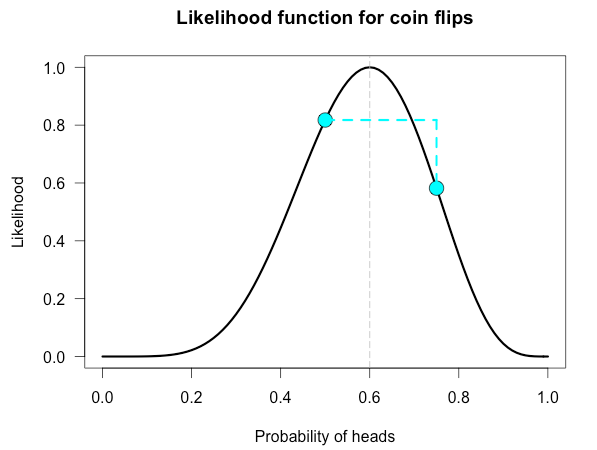
\includegraphics[width=0.8\textwidth]{pic/p05c03-snip01.png}
    \caption{Likelihood function for 6 heads in 10 flips}
    \label{fig:p05c03-snip01}
\end{figure}

The vertical dotted line marks the hypothesis best supported by the data. The likelihood ratio of any two hypotheses is simply the ratio of their heights on this curve. We can see from the plot that the fair coin has a higher likelihood than our trick coin.

How does the curve change if instead of 6 heads out of 10 tosses, we tossed 100 times and obtained 60 heads?

\begin{figure}[h]
    \centering
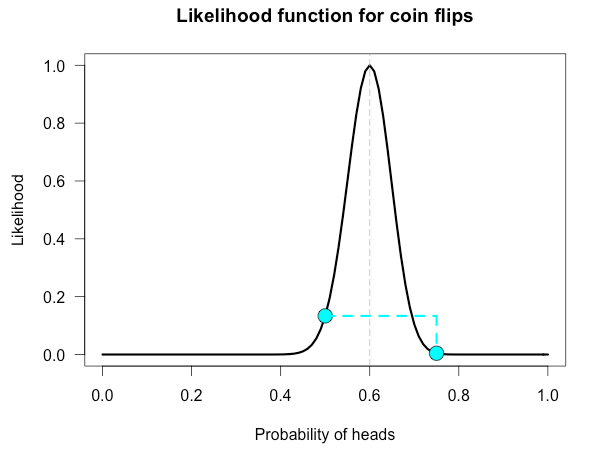
\includegraphics[width=.8\textwidth]{pic/p05c03-snip02.png}
    \caption{Likelihood function for  60 heads in 100  flips}
    \label{fig:p05c03-snip02}
\end{figure}

Our curve gets much narrower! How did the strength of evidence change for the fair coin vs the trick coin? The new likelihood ratio is $\mathrm{L}(.5) / \mathrm{L}(.75) \approx 29.9$. Much stronger evidence!\footnote{Obtaining 60 heads in 100 tosses is equivalent to obtaining 6 heads in 10 tosses 10 separate times. To obtain this new likelihood ratio we can simply multiply our ratios together. That is, raise the first ratio to the power of 10; $1.4^{\wedge} 10 \approx 28.9$, which is just slightly off from the correct value of 29.9 due to rounding.} However, due to the narrowing, neither of these hypothesized values are very high up on the curve anymore. It might be more informative to compare each of our hypotheses against the best supported hypothesis. This gives us two likelihood ratios: $\mathrm{L}(.6) / \mathrm{L}(.5) \approx 7.5$  and $\mathrm{L}(.6) / \mathrm{L}(.75) \approx 224$.

\begin{figure}[h]
    \centering
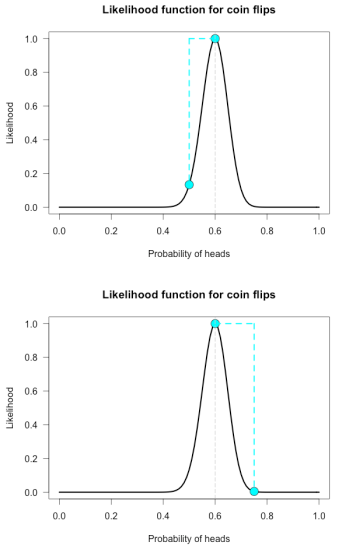
\includegraphics[width=0.8\textwidth]{pic/p05c03-snip03.png}
    \caption{Likelihood function ratios 7.5 and 224}
    \label{fig:p05c03-snip03}
\end{figure}

Here is one more curve, for when we obtain 300 heads in 500 coin flips.

\begin{figure}[h]
    \centering
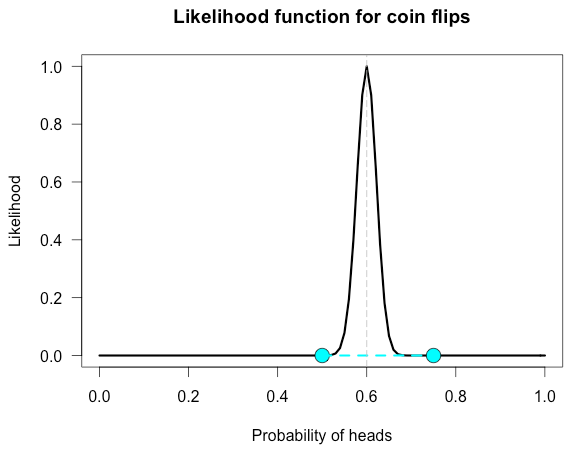
\includegraphics[width=0.8\textwidth]{pic/p05c03-snip04.png}
    \caption{Likelihood function for  300 heads in 500  flips}
    \label{fig:p05c03-snip04}
\end{figure}

Notice that both of our hypotheses look to be very near the minimum of the graph. Yet their likelihood ratio is much stronger than before. For this data the likelihood ratio$\mathrm{L}(.5) / \mathrm{L}(.75)$ is nearly \textbf{24 million!} The inherent relativity of evidence is made clear here: The fair coin was supported when compared to \textit{one particular} trick coin. But this should not be interpreted as absolute evidence for the fair coin, because the likelihood ratio for the maximally supported hypothesis vs the fair coin, $\mathrm{L}(.6) / \mathrm{L}(.5)$, is nearly \textbf{24 thousand!}

We need to be careful not to make blanket statements about absolute support, such as claiming that the maximum is ``strongly supported by the data''. Always ask, ``Compared to what?'' The best supported hypothesis will be only be weakly supported vs any hypothesis just before or just after it on the x-axis. For example, $\mathrm{L}(.6) / \mathrm{L}(.61) \approx 1.1$, which is barely any support one way or the other. It cannot be said enough that evidence for a hypothesis must be evaluated in consideration with a specific alternative.

\subsection{Connecting likelihood ratios to Bayes factors}

Bayes factors are simple extensions of likelihood ratios. A Bayes factor is a weighted average likelihood ratio based on the prior distribution specified for the hypotheses. (When the hypotheses are simple point hypotheses, the Bayes factor is equivalent to the likelihood ratio.) The likelihood ratio is evaluated at each point of the prior distribution and weighted by the probability we assign that value. If the prior distribution assigns the majority of its probability to values far away from the observed data, then the average likelihood for that hypothesis is lower than one that assigns probability closer to the observed data. In other words, you get a Bayes boost if you make more accurate predictions. Bayes factors are extremely valuable, and in a future post I will tackle the hard problem of assigning priors and evaluating weighted likelihoods.

I hope you come away from this post with a greater knowledge of, and appreciation for, likelihoods. Play around with the R code and you can get a feel for how the likelihood functions change for different data and different hypotheses of interest.


\begin{lstlisting}
## R code for the plots
## Plots the likelihood function for the data obtained
## h = number of successes (heads), n = number of trials (flips), 
## p1 = prob of success (head) on H1, p2 = prob of success (head) on H2
## Returns the likelihood ratio for p1 over p2. The default values are the ones used in the blog post
LR <- function(h,n,p1=.5,p2=.75){
        L1 <- dbinom(h,n,p1)/dbinom(h,n,h/n) ## Likelihood for p1, standardized vs the MLE
        L2 <- dbinom(h,n,p2)/dbinom(h,n,h/n) ## Likelihood for p2, standardized vs the MLE
        Ratio <- dbinom(h,n,p1)/dbinom(h,n,p2) ## Likelihood ratio for p1 vs p2
        curve((dbinom(h,n,x)/max(dbinom(h,n,x))), xlim = c(0,1), ylab = "Likelihood",xlab = "Probability of heads",las=1,
                main = "Likelihood function for coin flips", lwd = 3)
        points(p1, L1, cex = 2, pch = 21, bg = "cyan")
        points(p2, L2, cex = 2, pch = 21, bg = "cyan")
        lines(c(p1, p2), c(L1, L1), lwd = 3, lty = 2, col = "cyan")
        lines(c(p2, p2), c(L1, L2), lwd = 3, lty = 2, col = "cyan")
        abline(v = h/n, lty = 5, lwd = 1, col = "grey73")
        return(Ratio) ## Returns the likelihood ratio for p1 vs p2
}
\end{lstlisting}

Obtaining 60 heads in 100 tosses is equivalent to obtaining 6 heads in 10 tosses 10 separate times. To obtain this new likelihood ratio we can simply multiply our ratios together. That is, raise the first ratio to the power of 10; $1.4^{\wedge} 10 \approx 28.9$, which is just slightly off from the correct value of 29.9 due to rounding.

In the comments to the above blog, someone wrote:
`` Bayesian statistics is a religion that gives a false promise of certainty to believers in a world of uncertainty.''



\section{Updating priors via the likelihood}
\label{sec:Updatingpriorsviathelikelihood}

Taken from  \cite{etz2015d}.

Above I outlined the basic idea behind likelihoods and likelihood ratios. Likelihoods are relatively straightforward to understand because they are based on tangible data. Collect your data, and then the likelihood curve shows the relative support that your data lend to various simple hypotheses. Likelihoods are a key component of Bayesian inference because they are the bridge that gets us from prior to posterior.

In this post I explain how to use the likelihood to update a prior into a posterior. The simplest way to illustrate likelihoods as an updating factor is to use \textit{conjugate distribution families} \cite{Raiffa2000}. A prior and likelihood are said to be conjugate when the resulting posterior distribution is the same type of distribution as the prior. This means that if you have binomial data you can use a beta prior to obtain a beta posterior. If you had normal data you could use a normal prior and obtain a normal posterior. Conjugate priors are not required for doing Bayesian updating, but they make the calculations a lot easier so they are nice to use if you can.

I'll use some data from a recent NCAA 3-point shooting contest to illustrate how different priors can converge into highly similar posteriors.

\subsection{The data}

This year's NCAA shooting contest was a thriller that saw Cassandra Brown of the Portland Pilots win the grand prize. This means that she won the women's contest and went on to defeat the men's champion in a shoot-off. This got me thinking, just how good is Cassandra Brown?

What a great chance to use some real data in a toy example. She completed 4 rounds of shooting, with 25 shots in each round, for a total of 100 shots (I did the math). The data are counts, so I'll be using the binomial distribution as a data model (i.e., the likelihood). Her results were the following:
\begin{lstlisting}
Round 1: 13/25               
Round 2: 12/25               
Round 3: 14/25               
Round 4: 19/25
Total: 58/100
\end{lstlisting}
The likelihood curve below encompasses the entirety of statistical evidence that our 3-point data provide\footnote{I'm making a major assumption about the data: Any one shot is exchangeable with any other shot. This might not be defensible since the final ball on each rack is worth a bonus point, so maybe those shots differ systematically from regular shots, but it's a toy example so I'll ignore that possibility. There's also the possibility of her going on a hot streak, a.k.a. having a ``hot hand'', but I'm going to ignore that too because I'm the one writing this blog post and I want to keep it simple. There's also the possibility that she gets worse throughout the competition because she gets tired, but then there's also the possibility that she gets better as she warms up with multiple rounds. All of these things are reasonable to consider and I am going to ignore them all.}. The hypothesis with the most relative support is .58, and the curve is moderately narrow since there are quite a few data points. I didn't standardize the height of the curve in order to keep it comparable to the other curves I'll be showing.


\begin{figure*}[h]
\centering
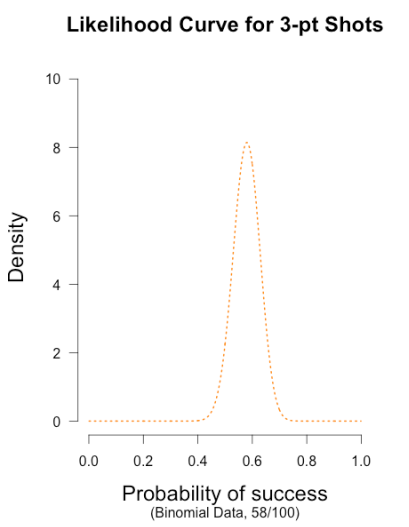
\includegraphics[width=0.4\textwidth]{pic/p05c03-snip05.png}
\caption{Likelihood for 3-pt Shots}
\label{fig:p05c03-snip05}
\end{figure*}

\FloatBarrier


\subsection{The prior}

Now the part that people often make a fuss about: choosing the prior. There are a few ways to choose a prior. Since I am using a binomial likelihood, I'll be using a conjugate beta prior. A beta prior has two shape parameters that determine what it looks like, and is denoted Beta($\alpha$, $\beta$). I like to think of priors in terms of what kind of information they represent. The shape parameters $\alpha$ and $\beta$ can be thought of as prior observations that I've made (or imagined).

Imagine my trusted friend caught the end of Brown's warm-up and saw her take two shots, making one and missing the other, and she tells me this information. This would mean I could reasonably use the common Beta(1, 1) prior, which represents a uniform density over [0, 1]. In other words, all possible values for Brown's shooting percentage are given equal weight before taking data into account, because the only thing I know about her ability is that both outcomes are possible\cite{LeeWagenmakers2005}.

Another common prior is called Jeffreys's prior, a Beta(1/2, 1/2) which forms a wide bowl shape. This prior would be recommended if you had extremely scarce information about Brown's ability. Is Brown so good that she makes nearly every shot, or is she so bad that she misses nearly every shot? This prior says that Brown's shooting rate is probably near the extremes, which may not necessarily reflect a reasonable belief for someone who is a college basketball player, but it has the benefit of having less influence on the posterior estimates than the uniform prior (since it is equal to 1 prior observation instead of 2). Jeffreys's prior is popular because it has some desirable properties, such as invariance under parameter transformation \cite{Jaynes2003}. So if instead of asking about Brown's shooting percentage I instead wanted to know her shooting percentage squared or cubed, Jeffreys's prior would remain the same shape while many other priors would drastically change shape.

Or perhaps I had another trusted friend who had arrived earlier and seen Brown take her final 13 shots in warm-up, and she saw 4 makes and 9 misses. Then I could use a Beta(4, 9) prior to characterize this prior information, which looks like a hump over .3 with density falling slowly as it moves outward in either direction. This prior has information equivalent to 13 shots, or roughly an extra 1/2 round of shooting.


\begin{figure}[h]
    \centering
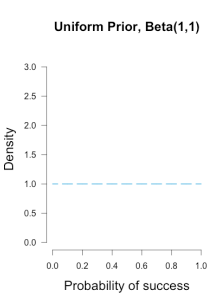
\includegraphics[width=0.3\textwidth]{pic/p05c03-snip06-1.png}
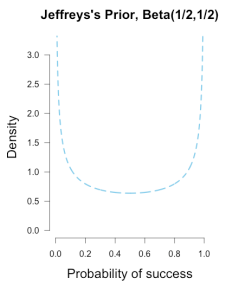
\includegraphics[width=0.3\textwidth]{pic/p05c03-snip06-2.png}
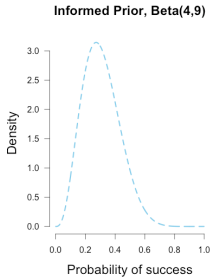
\includegraphics[width=0.3\textwidth]{pic/p05c03-snip06-3.png}
    \caption{Three different priors, or different Beta}
    \label{fig:p05c03-snip06}
\end{figure}

These are but three possible priors one could use. In your analysis you can use any prior you want, but if you want to be taken seriously you'd better give some justification for it. Bayesian inference allows many rules for prior construction.''This is my personal prior'' is a technically a valid reason, but if this is your only justification then your colleagues/reviewers/editors will probably not take your results seriously.

\FloatBarrier

\subsection{Updating the prior via the likelihood}

Now for the easiest part. In order to obtain a posterior, simply use Bayes's rule:

Posterior $\propto$ Likelihood $X$ Prior

The posterior is proportional to the likelihood multiplied by the prior. What's nice about working with conjugate distributions is that Bayesian updating really is as simple as basic algebra. We take the formula for the binomial likelihood, which from above is known to be:

Likelihood$=p^{x}(1-p)^{n-x}$

and then multiply it by the formula for the beta prior with $\alpha$ and $\beta$ shape parameters:

Prior$=p^{\alpha-1}(1-p)^{\beta-1}$ 

to obtain the following formula for the posterior:

Posterior $=p^{x}(1-p)^{n-x} p^{\alpha-1}(1-p)^{\beta-1}$

With a little bit of algebra knowledge, you'll know that multiplying together terms with the same base means the exponents can be added together. So the posterior formula can be rewritten as:

Posterior $=p^{x} p^{\alpha-1}(1-p)^{n-x}(1-p)^{\beta-1}$

and then by adding the exponents together the formula simplifies to:

Posterior $=p^{\alpha-1+x}(1-p)^{\beta-1+n-x}$

and it's that simple! Take the prior, add the successes and failures to the different exponents, and voila. The distributional notation is even simpler. Take the prior, Beta($\alpha$, $\beta$), and add the successes from the data, $x$, to $\alpha$ and the failures, $n – x$, to $\beta$, and there's your posterior, Beta($\alpha+x$, $\beta+n-x$).

Remember from the previous that likelihoods don't care about what order the data arrive in, it always results in the same curve. This property of likelihoods is carried over to posterior updating. The formulas above serve as another illustration of this fact. It doesn't matter if you add a string of six single data points, 1+1+1+1+1+1+1 or a batch of +6 data points; the posterior formula in either case ends up with 6 additional points in the exponents.

\subsection{Looking at some posteriors}

Back to Brown's shooting data. She had four rounds of shooting so I'll treat each round as a batch of new data. Her results for each round were: 13/25, 12/25, 14/25, 19/25. I'll show how the different priors are updated with each batch of data. A neat thing about Bayesian updating is that after batch 1 is added to the initial prior, its posterior is used as the prior for the next batch of data. And as the formulas above indicate, the order or frequency of additions doesn't make a difference on the final posterior. I'll verify this at the end of the post.

In the following plots, the prior is shown in blue (as above), the likelihood in orange (as above), and the resulting posteriors after Brown's first 13/25 makes in purple.


\begin{figure}[h]
    \centering
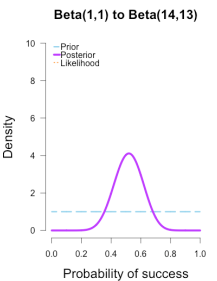
\includegraphics[width=0.3\textwidth]{pic/p05c03-snip07-1.png}
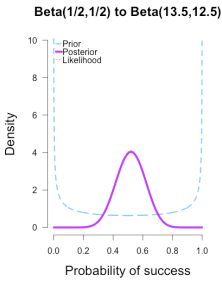
\includegraphics[width=0.3\textwidth]{pic/p05c03-snip07-2.png}
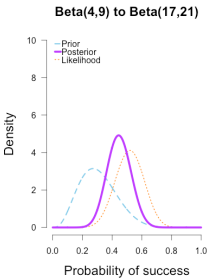
\includegraphics[width=0.3\textwidth]{pic/p05c03-snip07-3.png}
    \caption{Priors, likelihood and posteriors}
    \label{fig:p05c03-snip07}
\end{figure}

\FloatBarrier

In the first and second plot the likelihood is nearly invisible because the posterior sits right on top of it. When the prior has only 1 or 2 data points worth of information, it has essentially no impact on the posterior shape\footnote{There is a tendency to call any priors that have very little impact on the posterior ``non-informative'', but, as I mentioned in the section on determining priors, uniform priors that seem non-informative in one context can become highly informative with parameter transformation \cite{MuZhuLu2004}. Jeffreys's prior was derived precisely with that in mind, so it carries little information no matter what transformation is applied.} . The third plot shows how the posterior splits the difference between the likelihood and the informed prior based on the relative quantity of information in each.

The posteriors obtained from the uniform and Jeffreys's priors suggest the best guess for Brown's shooting percentage is around 50\%, whereas the posterior obtained from the informed prior suggests it is around 40\%. No surprise here since the informed prior represents another 1/2 round of shots where Brown performed poorly, which shifts the posterior towards lower values. But all three posteriors are still quite broad, and the breadth of the curves can be thought to represent the uncertainty in my estimates. More data $\rightarrow$ tighter curves $\rightarrow$ less uncertainty.

Now I'll add the second round performance as a new likelihood (12/25 makes), and I'll take the posteriors from the first round of updating as new priors for the second round of updating. So the purple posteriors from the plots above are now blue priors, the likelihood is orange again, and the new posteriors are purple.


\begin{figure}[h]
    \centering
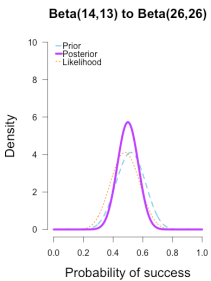
\includegraphics[width=0.3\textwidth]{pic/p05c03-snip08-1.png}
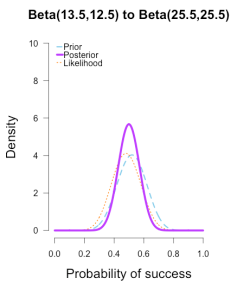
\includegraphics[width=0.3\textwidth]{pic/p05c03-snip08-2.png}
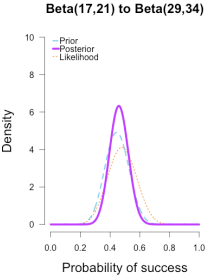
\includegraphics[width=0.3\textwidth]{pic/p05c03-snip08-3.png}
    \caption{Priors, likelihood and posteriors}
    \label{fig:p05c03-snip08}
\end{figure}


The left two plots look nearly identical, which should be no surprise since their posteriors were essentially equivalent after only 1 round of data updates. The third plot shows a posterior still slightly shifted to the left of the others, but it is much more in line with them than before. All three posteriors are getting narrower as more data is added.

The last two rounds of updating are shown below, again with posteriors from the previous round taken as priors for the next round. At this point they've all converged to very similar posteriors that are much narrower, translating to less uncertainty in my estimates.

\FloatBarrier


\begin{figure}[h]
    \centering
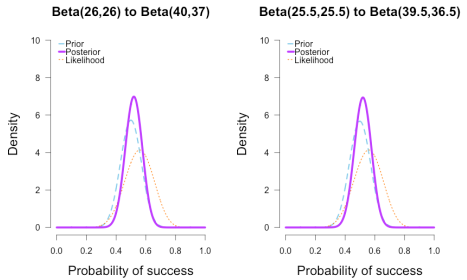
\includegraphics[width=0.6\textwidth]{pic/p05c03-snip09.png}
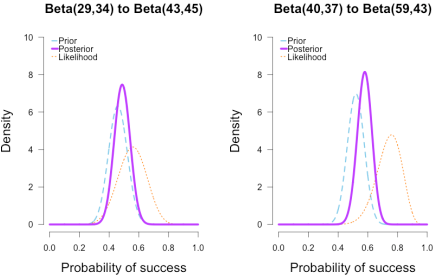
\includegraphics[width=0.6\textwidth]{pic/p05c03-snip10.png}
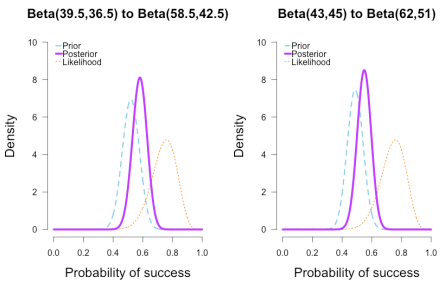
\includegraphics[width=0.6\textwidth]{pic/p05c03-snip11.png}
    \caption{Priors, likelihood and posteriors}
    \label{fig:p05c03-snip09}
\end{figure}

These posterior distributions look pretty similar now! Just as an illustration, I'll show what happens when I update the initial priors with all of the data at once.


\begin{figure}[h]
    \centering
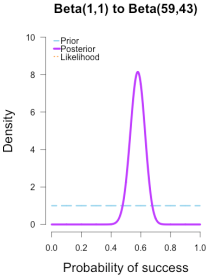
\includegraphics[width=0.3\textwidth]{pic/p05c03-snip12-1.png}
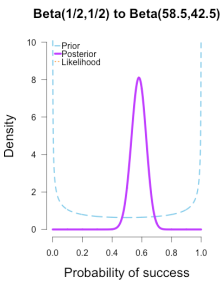
\includegraphics[width=0.3\textwidth]{pic/p05c03-snip12-2.png}
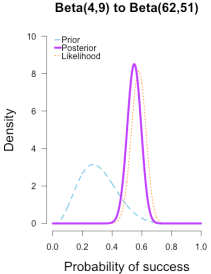
\includegraphics[width=0.3\textwidth]{pic/p05c03-snip12-3.png}
    \caption{Priors, likelihood and posteriors}
    \label{fig:p05c03-snip12}
\end{figure}

\FloatBarrier


As the formulas predict, the posteriors after one big batch of data are identical to those obtained by repeatedly adding multiple smaller batches of data. It's also a little easier to see the discrepancies between the final posteriors in this illustration because the likelihood curve acts as a visual anchor. The uniform and Jeffreys's priors result in posteriors that essentially fall right on top of the likelihood, whereas the informed prior results in a posterior that is very slightly shifted to the left of the likelihood.

My takeaway from these posteriors is that Cassandra Brown has a pretty damn good 3-point shot! In a future post I'll explain how to use this method of updating to make inferences using Bayes factors. It's called the Savage-Dickey density method, and I think it's incredibly intuitive and easy to use.
Notes:

\begin{lstlisting}
shotData<- c(1, 0, 0, 0, 1, 0, 1, 0, 1, 0, 0, 0, 1, 1, 1, 0, 1, 0, 1, 1, 1, 0, 0, 1, 1, 0, 0,
             1, 1, 1, 0, 0, 1, 1, 0, 0, 0, 1, 1, 1, 0, 0, 0, 0, 1, 1, 0, 1, 1, 0, 1, 0, 0, 1,
             0, 1, 0, 1, 1, 1, 0, 1, 0, 1, 0, 0, 1, 1, 0, 1, 0, 0, 1, 1, 1, 1, 1, 1, 1, 1, 1,
             1, 1, 1, 0, 0, 1, 1, 0, 0, 1, 1, 1, 0, 1, 1, 1, 1, 1, 0)

#figure 1 from blog, likelihood curve for 58/100 shots

x = seq(.001, .999, .001) ##Set up for creating the distributions
y2 = dbeta(x, 1 + 58, 1 + 42) # data for likelihood curve, plotted as the posterior from a beta(1,1)

plot(x, y2, xlim=c(0,1), ylim=c(0, 1.25 * max(y2,1.6)), type = "l", ylab= "Density", lty = 3,
     xlab= "Probability of success", las=1, main="Likelihood Curve for 3-pt Shots", sub= "(Binomial Data, 58/100)",lwd=2,
     cex.lab=1.5, cex.main=1.5, col = "darkorange", axes=FALSE)
axis(1, at = seq(0,1,.2)) #adds custom x axis
axis(2, las=1) # custom y axis

## Function for plotting priors, likelihoods, and posteriors for binomial data
## Output consists of a plot and various statistics
## PS and PF determine the shape of the prior distribution.
## PS = prior success, PF = prior failure for beta dist. 
## PS = 1, PF = 1 corresponds to uniform(0,1) and is default. If left at default, posterior will be equivalent to likelihood
## k = number of observed successes in the data, n = total trials. If left at 0 only plots the prior dist.
## null = Is there a point-null hypothesis? null = NULL leaves it out of plots and calcs
## CI = Is there a relevant X% credibility interval? .95 is recommended and standard

plot.beta <- function(PS = 1, PF = 1, k = 0, n = 0, null = NULL, CI = NULL, ymax = "auto", main = NULL) {
        
        x = seq(.001, .999, .001) ##Set up for creating the distributions
        y1 = dbeta(x, PS, PF) # data for prior curve
        y3 = dbeta(x, PS + k, PF + n - k) # data for posterior curve
        y2 = dbeta(x, 1 + k, 1 + n - k) # data for likelihood curve, plotted as the posterior from a beta(1,1)
        
        if(is.numeric(ymax) == T){ ##you can specify the y-axis maximum
                y.max = ymax
        }        
        else(
                y.max = 1.25 * max(y1,y2,y3,1.6) ##or you can let it auto-select
        )
        
        if(is.character(main) == T){
                Title = main
        }
        else(
                Title = "Prior-to-Posterior Transformation with Binomial Data"
        )
        
        
        plot(x, y1, xlim=c(0,1), ylim=c(0, y.max), type = "l", ylab= "Density", lty = 2,
             xlab= "Probability of success", las=1, main= Title,lwd=3,
             cex.lab=1.5, cex.main=1.5, col = "skyblue", axes=FALSE)
        
        axis(1, at = seq(0,1,.2)) #adds custom x axis
        axis(2, las=1) # custom y axis
        
        
        
        if(n != 0){
                #if there is new data, plot likelihood and posterior
                lines(x, y2, type = "l", col = "darkorange", lwd = 2, lty = 3)
                lines(x, y3, type = "l", col = "darkorchid1", lwd = 5)
                legend("topleft", c("Prior", "Posterior", "Likelihood"), col = c("skyblue", "darkorchid1", "darkorange"), 
                       lty = c(2,1,3), lwd = c(3,5,2), bty = "n", y.intersp = .55, x.intersp = .1, seg.len=.7)
                
                ## adds null points on prior and posterior curve if null is specified and there is new data
                if(is.numeric(null) == T){
                        ## Adds points on the distributions at the null value if there is one and if there is new data
                        points(null, dbeta(null, PS, PF), pch = 21, bg = "blue", cex = 1.5)
                        points(null, dbeta(null, PS + k, PF + n - k), pch = 21, bg = "darkorchid", cex = 1.5)
                        abline(v=null, lty = 5, lwd = 1, col = "grey73")
                        ##lines(c(null,null),c(0,1.11*max(y1,y3,1.6))) other option for null line
                }
        }
        
        ##Specified CI% but no null? Calc and report only CI
        if(is.numeric(CI) == T && is.numeric(null) == F){
                CI.low <- qbeta((1-CI)/2, PS + k, PF + n - k)
                CI.high <- qbeta(1-(1-CI)/2, PS + k, PF + n - k)
                
                SEQlow<-seq(0, CI.low, .001)
                SEQhigh <- seq(CI.high, 1, .001)
                ##Adds shaded area for x% Posterior CIs
                cord.x <- c(0, SEQlow, CI.low) ##set up for shading
                cord.y <- c(0,dbeta(SEQlow,PS + k, PF + n - k),0) ##set up for shading
                polygon(cord.x,cord.y,col='orchid', lty= 3) ##shade left tail
                cord.xx <- c(CI.high, SEQhigh,1) 
                cord.yy <- c(0,dbeta(SEQhigh,PS + k, PF + n - k), 0)
                polygon(cord.xx,cord.yy,col='orchid', lty=3) ##shade right tail
                
                return( list( "Posterior CI lower" = round(CI.low,3), "Posterior CI upper" = round(CI.high,3)))
        }
        
        ##Specified null but not CI%? Calculate and report BF only 
        if(is.numeric(null) == T && is.numeric(CI) == F){
                null.H0 <- dbeta(null, PS, PF)
                null.H1 <- dbeta(null, PS + k, PF + n - k)
                CI.low <- qbeta((1-CI)/2, PS + k, PF + n - k)
                CI.high <- qbeta(1-(1-CI)/2, PS + k, PF + n - k)
                return( list("BF01 (in favor of H0)" = round(null.H1/null.H0,3), "BF10 (in favor of H1)" = round(null.H0/null.H1,3)
                ))
        }
        
        ##Specified both null and CI%? Calculate and report both
        if(is.numeric(null) == T && is.numeric(CI) == T){
                null.H0 <- dbeta(null, PS, PF)
                null.H1 <- dbeta(null, PS + k, PF + n - k)
                CI.low <- qbeta((1-CI)/2, PS + k, PF + n - k)
                CI.high <- qbeta(1-(1-CI)/2, PS + k, PF + n - k)
                
                SEQlow<-seq(0, CI.low, .001)
                SEQhigh <- seq(CI.high, 1, .001)
                ##Adds shaded area for x% Posterior CIs
                cord.x <- c(0, SEQlow, CI.low) ##set up for shading
                cord.y <- c(0,dbeta(SEQlow,PS + k, PF + n - k),0) ##set up for shading
                polygon(cord.x,cord.y,col='orchid', lty= 3) ##shade left tail
                cord.xx <- c(CI.high, SEQhigh,1) 
                cord.yy <- c(0,dbeta(SEQhigh,PS + k, PF + n - k), 0)
                polygon(cord.xx,cord.yy,col='orchid', lty=3) ##shade right tail
                
                return( list("BF01 (in favor of H0)" = round(null.H1/null.H0,3), "BF10 (in favor of H1)" = round(null.H0/null.H1,3),
                             "Posterior CI lower" = round(CI.low,3), "Posterior CI upper" = round(CI.high,3)))
        }
        
}

#plot dimensions (415,550) for the blog figures

#Initial Priors
plot.beta(1,1,ymax=3.2,main="Uniform Prior, Beta(1,1)")
plot.beta(.5,.5,ymax=3.2,main="Jeffreys's Prior, Beta(1/2,1/2)")
plot.beta(4,9,ymax=3.2,main="Informed Prior, Beta(4,9)")

#Posteriors after Round 1
plot.beta(1,1,13,25,main="Beta(1,1) to Beta(14,13)",ymax=10)
plot.beta(.5,.5,13,25,main="Beta(1/2,1/2) to Beta(13.5,12.5)",ymax=10)
plot.beta(4,9,13,25,main="Beta(4,9) to Beta(17,21)",ymax=10)

#Posteriors after Round 2
plot.beta(14,13,12,25,ymax=10,main="Beta(14,13) to Beta(26,26)")
plot.beta(13.5,12.5,12,25,ymax=10,main="Beta(13.5,12.5) to Beta(25.5,25.5)")
plot.beta(17,21,12,25,ymax=10,main="Beta(17,21) to Beta(29,34)")

#Posteriors after Round 3
plot.beta(26,26,14,25,ymax=10,main="Beta(26,26) to Beta(40,37)")
plot.beta(25.5,25.5,14,25,ymax=10,main="Beta(25.5,25.5) to Beta(39.5,36.5)")
plot.beta(29,34,14,25,ymax=10,main="Beta(29,34) to Beta(43,45)")

#Posteriors after Round 4
plot.beta(40,37,19,25,ymax=10,main="Beta(40,37) to Beta(59,43)")
plot.beta(39.5,36.5,19,25,ymax=10,main="Beta(39.5,36.5) to Beta(58.5,42.5)")
plot.beta(43,45,19,25,ymax=10,main="Beta(43,45) to Beta(62,51)")

#Initial Priors and final Posteriors after all rounds at once
plot.beta(1,1,58,100,ymax=10,main="Beta(1,1) to Beta(59,43)")
plot.beta(.5,.5,58,100,ymax=10,main="Beta(1/2,1/2) to Beta(58.5,42.5)")
plot.beta(4,9,58,100,ymax=10,main="Beta(4,9) to Beta(62,51)")
\end{lstlisting}

\section{Visualization of the Bayes Factor}
\label{sec:VisualizationoftheBayesFactor}

Taken from  \cite{etz2015b}.

 In this post I'll explain how using Bayes factors for model comparison can be conceptualized as a simple extension of likelihood ratios.
There's that coin again

Imagine we're in a similar situation as before: I've flipped a coin 100 times and it came up 60 heads and 40 tails. The likelihood function for binomial data in general is:

\begin{equation}P(X=x) \propto p^{x}(1-p)^{n-x}\end{equation}

and for this particular result:

\begin{equation}P(X=60) \propto p^{60}(1-p)^{40}\end{equation}

The corresponding likelihood curve is shown below, which displays the relative likelihood for all possible simple (point) hypotheses given this data. Any likelihood ratio can be calculated by simply taking the ratio of the different hypotheses's heights on the curve.


\begin{figure}[h]
    \centering
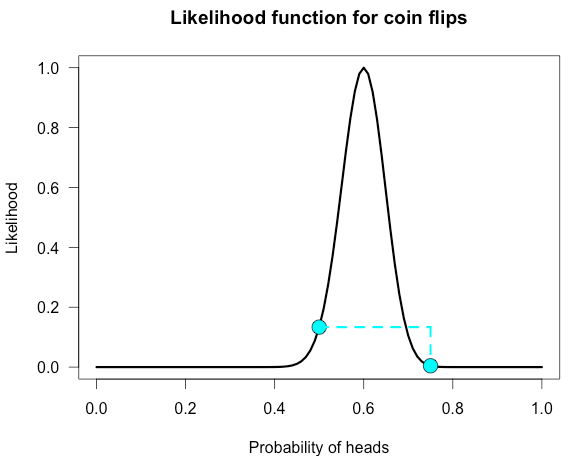
\includegraphics[width=0.6\textwidth]{pic/p05c03-snip13.png}
    \caption{Likelihood for coin flips}
    \label{fig:p05c03-snip13}
\end{figure}

In that previous section I compared the fair coin hypothesis H0: $P(H)$=.5 vs one particular trick coin hypothesis H1: $P(H)$=.75. For 60 heads out of 100 tosses, the likelihood ratio for these hypotheses is L(.5)/L(.75) = 29.9. This means the data are 29.9 times as probable under the fair coin hypothesis than  \textit{this particular trick}  coin hypothesis. But often we don't have theories precise enough to make point predictions about parameters, at least not in psychology. So it's often helpful if we can assign a \textit{range of plausible values} for parameters as dictated by our theories.

\subsection{Enter the Bayes factor}

Calculating a Bayes factor is a simple extension of this process. A Bayes factor is a weighted average likelihood ratio, where the weights are based on the prior distribution specified for the hypotheses. For this example I'll keep the simple fair coin hypothesis as the null hypothesis  H0: $P(H)$=.5  but now the alternative hypothesis will become a composite hypothesis\footnote{A lot of ink has been spilled arguing about how one should define $P(\Theta)$. I talked about it a little a previous post.}  H1: $P(\Theta)$. The likelihood ratio is evaluated at each point of $P(\Theta)$ and weighted by the relative plausibility we assign that value. Then once we've assigned weights to each ratio we just take the average to get the Bayes factor. Figuring out how the weights should be assigned (the prior) is the tricky part.

Imagine my composite hypothesis, $P(\Theta)$, is a combination of 21 different point hypotheses, all evenly spaced out between 0 and 1 and all of these points are weighted equally (not a very realistic hypothesis!). So we end up with $P(\Theta)$ = {0, .05, .10, .15, . . ., .9, .95, 1}. The likelihood ratio can be evaluated at every possible point hypothesis relative to H0, and we need to decide how to assign weights. This is easy for this $P(\Theta)$; we assign zero weight for every likelihood ratio that is not associated with one of the point hypotheses contained in $P(\Theta)$, and we assign weights of 1 to all likelihood ratios associated with the 21 points in $P(\Theta)$.

This gif has the 21 point hypotheses of $P(\Theta)$ represented as blue vertical lines (indicating where we put our weights of 1), and the turquoise tracking lines represent the likelihood ratio being calculated at every possible point relative to H0: $P(H)$=.5. (Remember, the likelihood ratio is the ratio of the heights on the curve.) This means we only care about the ratios given by the tracking lines when the dot attached to the moving arm aligns with the vertical $P(\Theta)$ lines. [edit: this paragraph added as clarification]

\begin{figure}[h]
    \centering
    \animategraphics[controls,width=\textwidth]{10}{pic/seqs/p05c03-snip14-}{0}{100}
    \caption{Likelihood for coin flips}
    \label{fig:p05c03-snip14}
\end{figure}
The 21 likelihood ratios associated with $P(\Theta)$ are:

{~0, ~0, ~0, ~0, ~0, ~0, ~0, ~0, .002, .08, 1, 4.5, 7.5, 4.4, .78, .03, ~0, ~0, ~0, ~0, ~0}

Since they are all weighted equally we simply average, and obtain BF = 18.3/21 = .87. In other words, the data (60 heads out of 100) are 1/.87 = 1.15 times more probable under the null hypothesis   H0: $P(H)$=.5   than this particular composite hypothesis H1: $P(\Theta)$. Entirely uninformative! Despite tossing the coin 100 times we have extremely weak evidence that is hardly worth even acknowledging. This happened because much of $P(\Theta)$ falls in areas of extremely low likelihood relative to H0, as evidenced by those 13 zeros above. $P(\Theta)$ is flexible, since it covers the entire possible range of $\Theta$, but this flexibility comes at a price. You have to pay for all of those zeros with a lower weighted average and a smaller Bayes factor.

Now imagine I had seen a trick coin like this before, and I know it had a slight bias towards landing heads. I can use this information to make more pointed predictions. Let's say I define $P(\Theta)$ as 21 equally weighted point hypotheses again, but this time they are all equally spaced between .5 and .75, which happens to be the highest density region of the likelihood curve (how fortuitous!). Now $P(\Theta)$ = {.50, .5125, .525, . . ., .7375, .75}.

\begin{figure}[h]
    \centering
    \animategraphics[controls,width=\textwidth]{10}{pic/seqs/p05c03-snip15-}{0}{100}
    \caption{Likelihood for coin flips}
    \label{fig:p05c03-snip15}
\end{figure}


The 21 likelihood ratios associated with the new $P(\Theta)$ are:

{1.00, 1.5, 2.1, 2.8, 4.5, 5.4, 6.2, 6.9, 7.5, 7.3, 6.9, 6.2, 4.4, 3.4, 2.6, 1.8, .78, .47, .27, .14, .03}

They are all still weighted equally, so the simple average is BF = 72/21 = 3.4. Three times more informative than before, and in favor of $P(\Theta)$ this time! \textit{And no zeros}. We were able to add theoretically relevant information to H1 to make more accurate predictions, and we get rewarded with a Bayes boost. (But this result is only 3-to-1 evidence, which is still fairly weak.)

This new $P(\Theta)$ is risky though, because if the data show a bias towards tails or a more extreme bias towards heads then it faces a very heavy penalty (many more zeros). High risk = high reward with the Bayes factor. Make pointed predictions that match the data and get a bump to your BF, but if you're wrong then pay a steep price. For example, if the data were 60 tails instead of 60 heads the BF would be 10-to-1 \textit{against} $P(\Theta)$ rather than 3-to-1 for $P(\Theta)$!

Now, typically people don't actually specify hypotheses like these. Typically they use continuous distributions, but the idea is the same. Take the likelihood ratio at each point relative to H0, weigh according to plausibilities given in $P(\Theta)$, and then average.

\subsection{A more realistic (?) example}

Imagine you're walking down the sidewalk and you see a shiny piece of foreign currency by your feet. You pick it up and want to know if it's a fair coin or an unfair coin. As a Bayesian you have to be precise about what you mean by fair and unfair. Fair is typically pretty straightforward   H0: $P(H)$=.5 as before   but unfair could mean anything. Since this is a completely foreign coin to you, you may want to be fairly open-minded about it. After careful deliberation, you assign $P(\Theta)$ a beta distribution, with shape parameters 10 and 10. That is, H1: $P(\Theta)$ $\approx$ Beta(10, 10). This means that if the coin isn't fair, it's probably close to fair but it could reasonably be moderately biased, and you have no reason to think it is particularly biased to one side or the other.


\begin{figure}[h]
    \centering
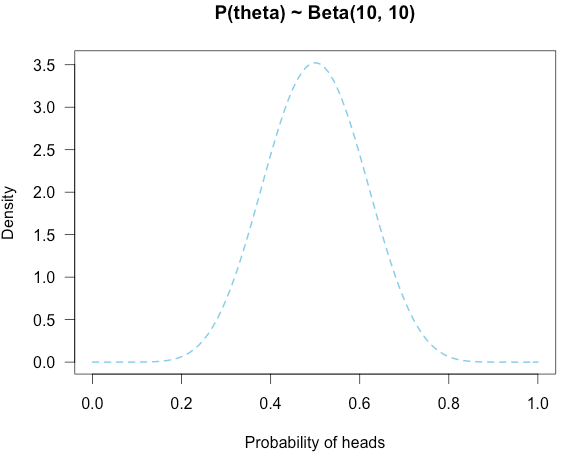
\includegraphics[width=0.6\textwidth]{pic/p05c03-snip16.png}
    \caption{Likelihood for coin flips}
    \label{fig:p05c03-snip16}
\end{figure}


Now you build a perfect coin-tosser machine and set it to toss 100 times (but not any more than that because you haven't got all day). You carefully record the results and the coin comes up 33 heads out of 100 tosses. Under which hypothesis are these data more probable, H0 or H1? In other words, which hypothesis did the better job predicting these data?

This may be a continuous prior but the concept is exactly the same as before: weigh the various likelihood ratios based on the prior plausibility assignment and then average. The continuous distribution on $P(\Theta)$ can be thought of as a set of many many point hypotheses spaced very very close together. So if the range of $\Theta$ we are interested in is limited to 0 to 1, as with binomials and coin flips, then a distribution containing 101 point hypotheses spaced .01 apart, can effectively be treated as if it were continuous. The numbers will be a little off but all in all it's usually pretty close. So imagine that instead of 21 hypotheses you have 101, and their relative plausibilities\footnote{I've rescaled the likelihood curve to match the scale of the prior density under H1. This doesn't affect the values of the Bayes factor or likelihood ratios because the scaling constant cancels itself out.} follow the shape of a Beta(10, 10). 


\begin{figure}[h]
    \centering
    \animategraphics[controls,width=\textwidth]{10}{pic/seqs/p05c03-snip17-}{0}{100}
    \caption{Likelihood for coin flips}
    \label{fig:p05c03-snip17}
\end{figure}



Since this is not a uniform distribution, we need to assign varying weights to each likelihood ratio. Each likelihood ratio associated with a point in $P(\Theta)$ is simply multiplied by the respective density assigned to it under $P(\Theta)$. For example, the density of $P(\Theta)$ at .4 is 2.44. So we multiply the likelihood ratio at that point, L(.4)/L(.5) = 128, by 2.44, and add it to the accumulating total likelihood ratio. Do this for every point and then divide by the total number of points, in this case 101, to obtain the approximate Bayes factor. The total weighted likelihood ratio is 5564.9, divide it by 101 to get 55.1, and there's the Bayes factor. In other words, the data are roughly 55 times more probable under this composite H1 than under H0. The alternative hypothesis H1 did a much better job predicting these data than did the null hypothesis H0.

The actual Bayes factor is obtained by integrating the likelihood with respect to H1's density distribution and then dividing by the (marginal) likelihood of H0. Essentially what it does is cut $P(\Theta)$ into slices infinitely thin before it calculates the likelihood ratios, re-weighs, and averages. That Bayes factor comes out to 55.7, which is basically the same thing we got through this ghetto visualization demonstration!
Take home

The take-home message is hopefully pretty clear at this point: When you are comparing a point null hypothesis with a composite hypothesis, the Bayes factor can be thought of as a weighted average of every point hypothesis's likelihood ratio against H0, and the weights are determined by the prior density distribution of H1. Since the Bayes factor is a weighted average based on the prior distribution, it's really important to think hard about the prior distribution you choose for H1. In a previous post, I showed how different priors can converge to the same posterior with enough data. The priors are often said to ``wash out'' in estimation problems like that. This is not necessarily the case for Bayes factors. The priors you choose matter, so think hard!


\begin{lstlisting}
## Plots the likelihood function for the data obtained
## h = number of successes (heads), n = number of trials (flips), 
## p1 = prob of success (head) on H1, p2 = prob of success (head) on H0
#the auto plot loop is taken from http://www.r-bloggers.com/automatically-save-your-plots-to-a-folder/
#and then the pngs are combined into a gif online 


LR <- function(h,n,p1=seq(0,1,.01),p2=rep(.5,101)){
        L1 <- dbinom(h,n,p1)/dbinom(h,n,h/n) ## Likelihood for p1, standardized vs the MLE
        L2 <- dbinom(h,n,p2)/dbinom(h,n,h/n) ## Likelihood for p2, standardized vs the MLE
        Ratio <<- dbinom(h,n,p1)/dbinom(h,n,p2) ## Likelihood ratio for p1 vs p2, saves to global workspace with <<-
        x<- seq(0,1,.01) #sets up for loop
        m<- seq(0,1,.01) #sets up for p(theta)
        ym<-dbeta(m,10,10) #p(theta) densities
        names<-seq(1,length(x),1) #names for png loop
        for(i in 1:length(x)){
                mypath<-file.path("~","Dropbox","Blog Drafts","bfs","figs1",paste("myplot_", names[i], ".png", sep = "")) #set up for save file path
                png(file=mypath, width=1200,height=1000,res=200) #the next plotted item saves as this png format
                curve(3.5*(dbinom(h,n,x)/max(dbinom(h,n,h/n))), ylim=c(0,3.5), xlim = c(0,1), ylab = "Likelihood",
                      xlab = "Probability of heads",las=1, main = "Likelihood function for coin flips", lwd = 3)
                
                lines(m,ym, type="h", lwd=1, lty=2, col="skyblue" ) #p(theta) density
                
                points(p1[i], 3.5*L1[i], cex = 2, pch = 21, bg = "cyan") #tracking dot
                points(p2, 3.5*L2, cex = 2, pch = 21, bg = "cyan") #stationary null dot
                #abline(v = h/n, lty = 5, lwd = 1, col = "grey73") #un-hash if you want to add a line at the MLE
                
                lines(c(p1[i], p1[i]), c(3.5*L1[i], 3.6), lwd = 3, lty = 2, col = "cyan") #adds vertical line at p1
                lines(c(p2[i], p2[i]), c(3.5*L2[i], 3.6), lwd = 3, lty = 2, col = "cyan") #adds vertical line at p2, fixed at null
                lines(c(p1[i], p2[i]), c(3.6, 3.6), lwd=3,lty=2,col="cyan") #adds horizontal line connecting them
                dev.off() #lets you save directly
                }
}

LR(33,100) #executes the final example
v<-seq(0,1,.05) #the segments of P(theta) when it is uniform
sum(Ratio[v]) #total weighted likelihood ratio
mean(Ratio[v]) #average weighted likelihood ratio (i.e., BF)

x<- seq(0,1,.01) #segments for p(theta)~beta
y<-dbeta(x,10,10) #assigns densitys for P(theta)
k=sum(y*Ratio) #multiply likelihood ratios by the density under P(theta)
l=k/101 #weighted average likelihood ratio (i.e., BF)
\end{lstlisting}





\section{Evidence vs. Conclusions}
\label{sec:Evidencevs.Conclusions}

Taken from  \cite{etz2015c}.

\subsection{Perspective}

In this installment of Understanding Bayes I want to discuss the nature of Bayesian evidence and conclusions. In a previous post I focused on Bayes factors' mathematical structure and visualization. In this post I hope to give some idea of how Bayes factors should be interpreted \textit{in context}. How do we use the Bayes factor to come to a conclusion?

\subsection{How to calculate a Bayes factor}

I'm going to start with an example to show the nature of the Bayes factor. Imagine I have 2 baskets with black and white balls in them. In basket A there are 5 white balls and 5 black balls. In basket B there are 10 white balls. Other than the color, the balls are completely indistinguishable. Here's my advanced high-tech figure depicting the problem.

\begin{figure}[h]
\centering
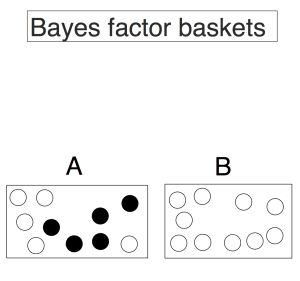
\includegraphics[width=0.3\textwidth]{pic/p05c03-snip17.png}
\caption{Bayes factor baskets}
\label{fig:p05c03-snip17}
\end{figure}

You choose a basket and bring it to me. The baskets aren't labeled so I can't tell by their appearance which one you brought. You tell me that in order to figure out which basket I have, I am allowed to take a ball out one at a time and then return it and reshuffle the balls around. What outcomes are possible here? In this case it's super simple: I can either draw a white ball or a black ball.

If I draw a black ball I immediately know I have basket A, since this is impossible in basket B. If I draw a white ball I can't rule anything out, but drawing a white ball counts as evidence for basket B over basket A. Since the white ball occurs with probability 1 if I have basket B, and probability .5 if I have basket A, then due to what is known as the Likelihood Axiom, I have evidence for basket B over basket A by a factor of 2.  See this post for a refresher on likelihoods, including the concepts such as the law of likelihood and the likelihood principle. The short version is that observations count as evidence for basket B over basket A if they are more probable given basket B than basket A.

\begin{figure}[h]
\centering
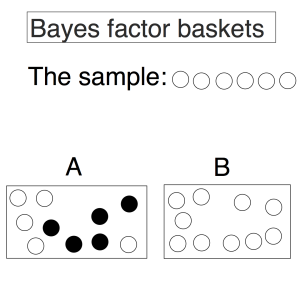
\includegraphics[width=0.3\textwidth]{pic/p05c03-snip18.png}
\caption{Bayes factor baskets}
\label{fig:p05c03-snip18}
\end{figure}

I continue to sample, and end up with this set of observations: {W, W, W, W, W, W}. Each white ball that I draw counts as evidence of 2 for basket B over basket A, so my evidence looks like this: {2, 2, 2, 2, 2, 2}. Multiply them all together and my total evidence for B over A is $2^6$, or 64. This interpretation is simple: The total accumulated data are, all together, 64 times more probable under basket B than basket A. This number represents a simple Bayes factor, or likelihood ratio.

\subsection{How to interpret a Bayes factor}

In one sense, the Bayes factor always has the same interpretation in every problem: It is a ratio formed by the probability of the data under each hypothesis. It's all about prediction. The bigger the Bayes factor the more one hypothesis outpredicted the other.

But in another sense the interpretation, and our reaction, necessarily depends on the context of the problem, and that is represented by another piece of the Bayesian machinery: The prior odds. The Bayes factor is the factor by which the data shift the balance of evidence from one hypothesis to another, and thus the amount by which the prior odds shift to posterior odds.

Imagine that before you brought me one of the baskets you told me you would draw a card from a standard, shuffled deck of cards. You have a rule: Bring me basket B if the card drawn is a black suit and bring basket A if it is a red suit. You pick a card and, without telling me what it was, bring me a basket. Which basket did you bring me? What information do I have about the basket before I get to draw a sample from it?

I know that there is a 50\% chance that you choose a black card, so there is a 50\% chance that you bring me basket B. Likewise for basket A. The prior probabilities in this scenario are 50\% for each basket, so the prior odds for basket A vs basket B are 1-to-1. (To calculate odds you just divide the probability of one hypothesis by the other.)


\begin{figure}[h]
\centering
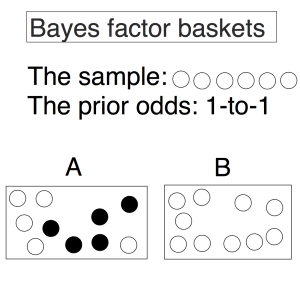
\includegraphics[width=0.3\textwidth]{pic/p05c03-snip19.png}
\caption{Bayes factor baskets}
\label{fig:p05c03-snip19}
\end{figure}

Let's say we draw our sample and get the same results as before: {W, W, W, W, W, W}. The evidence is the same: {2, 2, 2, 2, 2, 2} and the Bayes factor is the same, $2^6$=64. What do we conclude from this? Should we conclude we have basket A or basket B?

The conclusion is not represented by the Bayes factor, but by the posterior odds. The Bayes factor is just one piece of the puzzle, namely the evidence contained in our sample. In order to come to a conclusion the Bayes factor has to be combined with the prior odds to obtain posterior odds. We have to take into account the information we had before we started sampling. I repeat: The posterior odds are where the conclusion resides. Not the Bayes factor.

\subsection{Posterior odds (or probabilities) and conclusions}

In the example just given, the posterior odds happen to equal the Bayes factor. Since the prior odds were 1-to-1, we multiply by the Bayes factor of 1-to-64, to obtain posterior odds of 1-to-64 favoring basket B. This means that, when these are the only two possible baskets, the probability of basket A has shrunk from 50\% to 2\% and the probability of basket B has grown from 50\% to 98\%. (To convert odds to probabilities divide the odds by odds+1.) This is the conclusion, and it necessarily depends on the prior odds we assign. 

\begin{figure}[h]
\centering
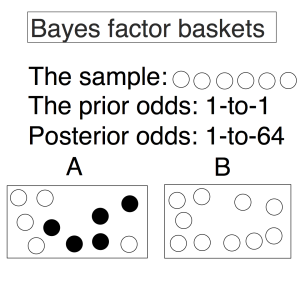
\includegraphics[width=0.3\textwidth]{pic/p05c03-snip20.png}
\caption{Bayes factor baskets}
\label{fig:p05c03-snip20}
\end{figure}


Say you had a different rule for picking the baskets. Let's say that this time you draw a card and bring me basket B if you draw a King (of any suit) and you bring me basket A if you draw any other card. Now the prior odds are 48-to-4, or 12-to-1, in favor of basket A.

The data from our sample are the same, {W, W, W, W, W, W}, and so is the Bayes factor, $2^6$= 64. The conclusion is qualitatively the same, with posterior odds of 1-to-5.3 that favor basket B. This means that, again when considering these as the only two possible baskets, the probability of basket A has been shrunk from 92\% to 16\% and the probability of basket B has grown from 8\% to 84\%. The Bayes factor is the same, but we are less confident in our conclusion. The prior odds heavily favored basket A, so it takes more evidence to overcome this handicap and reach as strong a conclusion as before.

\begin{figure}[h]
\centering
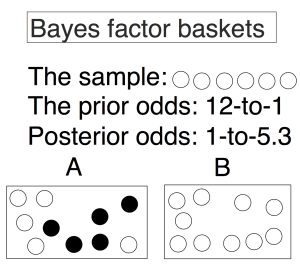
\includegraphics[width=0.3\textwidth]{pic/p05c03-snip21.png}
\caption{Bayes factor baskets}
\label{fig:p05c03-snip21}
\end{figure}


What happens when we change the rule once again: Bring me basket B if you draw a King of Hearts and basket A if you draw any other card. Now the prior odds are 51-to-1 in favor of basket A. The data are the same again, and the Bayes factor is still 64. Now the posterior odds are 1-to-1.3 in favor of basket B. This means that the probability of basket A has been shrunk from 98\% to 43\% and the probability of basket B has grown from 2\% to 57\%. The evidence, and the Bayes factor, is exactly the same — but the conclusion is totally ambiguous. 


\begin{figure}[h]
\centering
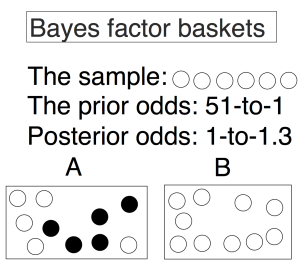
\includegraphics[width=0.3\textwidth]{pic/p05c03-snip22.png}
\caption{Bayes factor baskets}
\label{fig:p05c03-snip22}
\end{figure}


\subsection{Evidence vs. Conclusions}

In each case I've considered, the evidence has been exactly the same: 6 draws, all white. As a corollary to the discussion above, if you try to come to conclusions based only on the Bayes factor then you are implicitly assuming prior odds of 1-to-1. I think this is unreasonable in most circumstances. When someone looks at a medium-to-large Bayes factor in a study claiming ``sadness impairs color perception'' (or some other ‘cute' metaphor study published in Psych Science) and thinks, ``I don't buy this,'' they are injecting their prior odds into the equation. Their implicit conclusion is: ``My posterior odds for this study are not favorable.'' This is the conclusion. The Bayes factor is not the conclusion.

Many studies follow-up on earlier work, so we might give favorable prior odds; thus, when we see a Bayes factor of 5 or 10 we ``buy what the study is selling,'' so to speak. Or the study might be testing something totally new, so we might give unfavorable prior odds; thus, when we see a Bayes factor of 5 or 10 we remain skeptical. This is just another way of saying that we may reasonably require more evidence for extraordinary claims.

\subsection{When to stop collecting data}

It also follows from the above discussion that sometimes enough is enough. What I mean is that sometimes the conclusion for any reasonable prior odds assignment is strong enough that collecting more data is not worth the time, money, or energy. In the Bayesian framework the stopping rules don't affect the Bayes factor, and subsequently they don't affect the posterior odds. Take the second example above, where you gave me basket B if you drew any King. I had prior odds of 12-to-1 in favor of basket A, drew 6 white balls in a row, and ended up with 1-to-5.3 posterior odds in favor of basket B. This translated to a posterior probability of 84\% for basket B. If I draw 2 more balls and they are both white, my Bayes factor increases to $2^8$=256 (and this should not be corrected for multiple comparisons or so-called ``topping up''). My posterior odds increase to roughly 1-to-21 in favor of basket B, and the probability for basket B shoots up from 84\% to 99\%. I would say that's enough data for me to make a firm conclusion. But someone else might have other relevant information about the problem I'm studying, and they can come to a different conclusion.

\subsection{Conclusions are personal}

There's no reason another observer has to come to the same conclusion as me. She might have talked to you and you told her that you actually drew three cards (with replacement and reshuffle) and that you would only have brought me basket B if you drew three kings in a row. She has different information than I do, so naturally she has different prior odds (1728-to-1 in favor of basket A). She would come to a different conclusion than I would, namely that I was actually probably sampling from basket A — her posterior odds are roughly 7-to-1 in favor of basket A. We use the same evidence, a Bayes factor of $2^8$=256, but come to different conclusions. 

Conclusions are personal. I can't tell you what to conclude because I don't know all the information you have access to. But I can tell you what the evidence is, and you can use that to come to your own conclusion. In this post I used a mechanism to generate prior odds that are intuitive and obvious, but we come to our scientific judgments through all sorts of ways that aren't always easily expressed or quantified. The idea is the same however you come to your prior odds: If you're skeptical of a study that has a large Bayes factor, then you assigned it strongly unfavorable prior odds.

This is why I, and other Bayesians, advocate for reporting the Bayes factor in experiments. It is not because it tells someone what to conclude from the study, but that it lets them take the information contained in your data to come to their own conclusion. When you report your own Bayes factors for your experiments, in your discussion you might consider how people with different prior odds will react to your evidence. If your Bayes factor is not strong enough to overcome a skeptic's prior odds, then you may consider collecting more data until it is. If you're out of resources and the Bayes factor is not strong enough to overcome the prior odds of a moderate skeptic, then there is nothing wrong with acknowledging that other people may reasonably come to different conclusions about your study. Isn't that how science works?

\subsection{Bottom line}

If you want to come to a conclusion you need the posterior. If you want to make predictions about future sampling you need the posterior. If you want to make decisions you need the posterior (and a utility function; a topic for future blog). If you try to do all this with only the Bayes factor then you are implicitly assuming equal prior odds — which I maintain are almost never appropriate. (Insofar as you do ignore the prior and posterior, then do not be surprised when your Bayes factor simulations find strange results.) In the Bayesian framework each piece has its place. Bayes factors are an important piece of the puzzle, but they are not the only piece. They are simply the most basic piece from my perspective (after the sum and product rules) because they represent the evidence you accumulated in your sample. When you need to do something other than summarize evidence you have to expand your statistical arsenal.

For more introductory material on Bayesian inference, see the Understanding Bayes hub here.

\subsection{Technical caveat}

It's important to remember that everything is relative and conditional in the Bayesian framework. The posterior probabilities I mention in this post are simply the probabilities of the baskets under the assumption that those are the only relevant hypotheses. They are not absolute probabilities. In other words, instead of writing the posterior probability as P(H|D), it should really be written P(H|D,M), where M is the conditional that the only hypotheses considered are in the following model index: M= {A, B, … K). This is why I personally prefer to use odds notation, since it makes the relativity explicit.


\section{How to become a Bayesian in eight easy steps}
\label{sec:HowtobecomeaBayesianineighteasysteps}

Taken from  \cite{etz2016a}. 

We wrote an annotated reading list to get you started in learning Bayesian statistics \cite{etz2018a}.

It can be hard to know where to start when you want to learn about Bayesian statistics. I am frequently asked to share my favorite introductory resources to Bayesian statistics, and my go-to answer has been to share a dropbox folder with a bunch of PDFs that aren't really sorted or cohesive. In some sense I was acting as little more than a glorified Google Scholar search bar.

It seems like there is some tension out there with regard to Bayes, in that many people want to know more about it, but when they pick up, say, Andrew Gelman and colleagues' \textit{Bayesian Data Analysis} they get totally overwhelmed. And then they just think, ``Screw this esoteric B.S.'' and give up because it doesn't seem like it is worth their time or effort.

I think this happens a lot. Introductory Bayesian texts usually assume a level of training in mathematical statistics that most researchers simply don't have time (or otherwise don't need) to learn. There are actually a lot of accessible Bayesian resources out there that don't require much math stat background at all, but it just so happens that they are not consolidated anywhere so people don't necessarily know about them.

\subsection{Enter the eight step program}

Beth Baribault, Peter Edelsbrunner (@peter1328), Fabian Dablander (@fdabl), Quentin Gronau, and I have just finished a new paper \cite{etz2018a} that tries to remedy this situation, titled, ``How to become a Bayesian in eight easy steps: An annotated reading list.'' 
 Each paper in the special issue addresses a specific question we often hear about Bayesian statistics, and ours was the following:

\begin{quote}
    I am a reviewer/editor handling a manuscript that uses Bayesian methods; which articles should I read to get a quick idea of what that means?
\end{quote}

So the paper‘s goal is not so much to teach readers how to actually perform Bayesian data analysis — there are other papers in the special issue for that — but to facilitate readers in their quest to understand basic Bayesian concepts. We think it will serve as a nice introductory reading list for any interested researcher.

The format of the paper is straightforward. We highlight eight papers that had a big impact on our own understanding of Bayesian statistics, as well as short descriptions of an additional 28 resources in the \textit{Further reading} appendix. The first four papers are focused on theoretical introductions, and the second four have a slightly more applied focus.

We also give every resource a ranking from 1–9 on two dimensions: Focus (theoretical vs. applied) and Difficulty (easy vs. hard). We tried to provide a wide range of resources, from easy applications (\#14: Wagenmakers, Lee, and Morey's ``Bayesian benefits for the pragmatic researcher'') to challenging theoretical discussions (\#12: Edwards, Lindman and Savage's ``Bayesian statistical inference for psychological research'') and others in between.

The figure below  summarizes our rankings:

\begin{figure}[h]
\centering
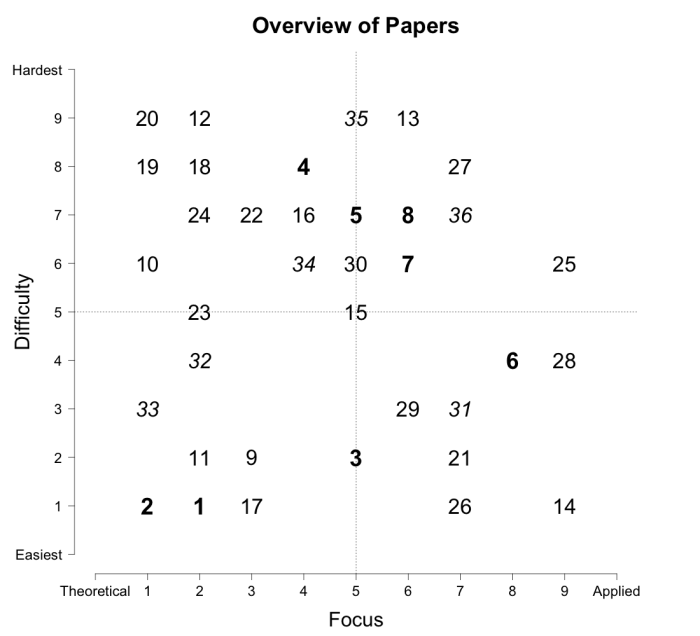
\includegraphics[width=0.3\textwidth]{pic/p05c03-snip23.png}
\caption{Reading list}
\label{fig:p05c03-snip23}
\end{figure}


The emboldened numbers (1–8) are the papers that we've commented on in detail, numbers in light text (9–30) are papers we briefly describe in the appendix, and the italicized numbers (31–36) are our recommended introductory books (also listed in the appendix).

This is how we chose to frame the paper,

\begin{quote}
    Overall, the guide is designed such that a researcher might be able to read all eight of the highlighted articles and some supplemental readings within a few days. After readers acquaint themselves with these sources, they should be well-equipped both to interpret existing research and to evaluate new research that relies on Bayesian methods.
\end{quote}

\subsection{The list}

Here's the list of papers we chose to cover in detail:

\begin{enumerate}
\item Lindley (1993) \cite{Lindley1993} The analysis of experimental data: The appreciation of tea and wine.

\item Kruschke (2015) \cite{Kruschke2015} chapter 2: Introduction: Credibility, models, and parameters.

\item Dienes (2011) \cite{Dienes2011}: Bayesian versus orthodox statistics: Which side are you on?

\item Rouder, Speckman, Sun, Morey, \& Iverson (2009) \cite{Rouder2009}: Bayesian t tests for accepting and rejecting the null hypothesis.

\item Vandekerckhove, Matzke, \& Wagenmakers (2014) \cite[Chapter 14]{Busemeyer2015}: Model comparison and the principle of parsimony. 

\item van de Schoot, Kaplan, Denissen, Asendorpf, Neyer, \& Aken (2014) \cite{vandeSchoot2013,ZondervanZwijnenburg2017}: A gentle introduction to Bayesian analysis: Applications to developmental research.
    
    
    
\item Lee and Vanpaemel \cite{LeeVanpaemel2017}: Determining priors for cognitive models.

\item Lee (2008) \cite{MdLee2008}: Three case studies in the Bayesian analysis of cognitive models.
\end{enumerate}


You'll have to check out the paper to see our commentary and to find out what other articles we included in the \textit{Further reading} appendix. We provide urls (web archived when possible; \lstinline{archive.org/web/}) to PDFs of the eight main papers (except \#2, that's on the DBDA website), and wherever possible for the rest of the resources (some did not have free copies online; see the References).

I thought this was a fun paper to write, and if you think you might want to learn some Bayesian basics I hope you will consider reading it.
